\iffalse
\documentclass[12pt]{article}
\usepackage{graphicx}
\usepackage[none]{hyphenat}
\usepackage{graphicx}
\usepackage{listings}
\usepackage[english]{babel}
\usepackage{graphicx}
\usepackage{caption} 
\usepackage{booktabs}
\usepackage{array}
\usepackage{amssymb} % for \because
\usepackage{amsmath}   % for having text in math mode
\usepackage{extarrows} % for Row operations arrows
\usepackage{listings}
\lstset{
  frame=single,
  breaklines=true
}
\usepackage{hyperref}
  
%Following 2 lines were added to remove the blank page at the beginning
\usepackage{atbegshi}% http://ctan.org/pkg/atbegshi
\AtBeginDocument{\AtBeginShipoutNext{\AtBeginShipoutDiscard}}
\usepackage{gensymb}


%New macro definitions
\newcommand{\mydet}[1]{\ensuremath{\begin{vmatrix}#1\end{vmatrix}}}
\providecommand{\brak}[1]{\ensuremath{\left(#1\right)}}
\providecommand{\sbrak}[1]{\ensuremath{{}\left[#1\right]}}
\providecommand{\norm}[1]{\left\lVert#1\right\rVert}
\providecommand{\abs}[1]{\left\vert#1\right\vert}
\newcommand{\solution}{\noindent \textbf{Solution: }}
\newcommand{\myvec}[1]{\ensuremath{\begin{pmatrix}#1\end{pmatrix}}}
\let\vec\mathbf


\begin{document}

\begin{center}
\title{\textbf{Lagrange Multipliers}}
\date{\vspace{-5ex}} %Not to print date automatically
\maketitle
\end{center}
\setcounter{page}{1}

\section{11$^{th}$ Maths - Chapter 10}
This is Problem-3.1 from Exercise 10.3 
\begin{enumerate}

\solution 

The equation of the given line is 
\begin{align}
	\myvec{1 \\ -\sqrt{3}}^\top\vec{x}+8 &= 0
\end{align}
Let $\vec{O}$ be the point from where we have to find the perpendicular distance. The perpendicular distance will be the minimum distance from $\vec{O}$ to the line. Let $\vec{P}$ be the foot of the perpendicular. 
\fi
		The given  problem can be formulated as 
\begin{align}
	\label{eq:11/10/3/3/1/lagmul/Eq3}
	\min_{\vec{x}} f\brak{\vec{x}} &= \norm{\vec{x}-\vec{O}}^2\\
	\text{s.t.} \quad g\brak{\vec{x}} = \vec{n}^T\vec{x}-c &= 0 
	\label{eq:11/10/3/3/1/lagmul/Eq1}
\end{align}
where
\begin{align}
	\vec{n} = \myvec{1 \\ -\sqrt{3}},\, 
	\vec{O} = \myvec{0 \\ 0},\,
	\text{ and } c = -8
\end{align}
Define
\begin{align}
	H\brak{\vec{x}, \lambda} &= f\brak{\vec{x}} - \lambda g\brak{\vec{x}} 
\end{align}
and we find that 
\begin{align}
	\nabla f\brak{\vec{x}} &= 2\brak{\vec{x}-\vec{O}} \\
        \nabla g\brak{\vec{x}} &= \vec{n}
\end{align}
We have to find $\lambda \in \mathbb{R}$ such that
\begin{align}
	&\nabla H\brak{\vec{x},\lambda} = 0 \\
        \label{eq:11/10/3/3/1/lagmul/Eqlambda}
	&\implies 2\brak{\vec{x}-\vec{O}} - \lambda\vec{n} = 0 \\
        \label{eq:11/10/3/3/1/lagmul/Eqx}
	&\implies \vec{x} = \frac{\lambda}{2}\vec{n} + \vec{O} 
\end{align}
Substituting \eqref{eq:11/10/3/3/1/lagmul/Eqx} in \eqref{eq:11/10/3/3/1/lagmul/Eq1}
\begin{align}
	\vec{n}^\top\brak{\frac{\lambda}{2}\vec{n} + \vec{O}}-c &= 0 \\
	\implies \lambda &= \frac{2\brak{c-\vec{n}^\top\vec{O}}}{\norm{\vec{n}}^2}
\end{align}
Substituting the value of $\lambda$ in \eqref{eq:11/10/3/3/1/lagmul/Eqlambda}, 
\begin{align}
	\vec{x}_{min} &= \vec{P} = \vec{O}+ \frac{\vec{n}\brak{c-\vec{n}^\top\vec{O}}}{\norm{\vec{n}}^2}\\
	&= \myvec{0 \\0}+ \frac{\myvec{1 \\ -\sqrt{3}}\brak{-8-\myvec{1 & -\sqrt{3}}\myvec{0 \\0}}}{4} \\
	&= \myvec{-2 \\ 2\sqrt{3}} \\
	OP &= \norm{\vec{P}-\vec{O}}^2 \\ 
	&= \norm{\myvec{-2 \\ 2\sqrt{3}}-\myvec{0 \\ 0}} \\
	&=  4
\end{align}	
The relevant figure is shown in \ref{fig:11/10/3/3/1/lagmul/Fig1}
\begin{figure}[!h]
	\begin{center}
		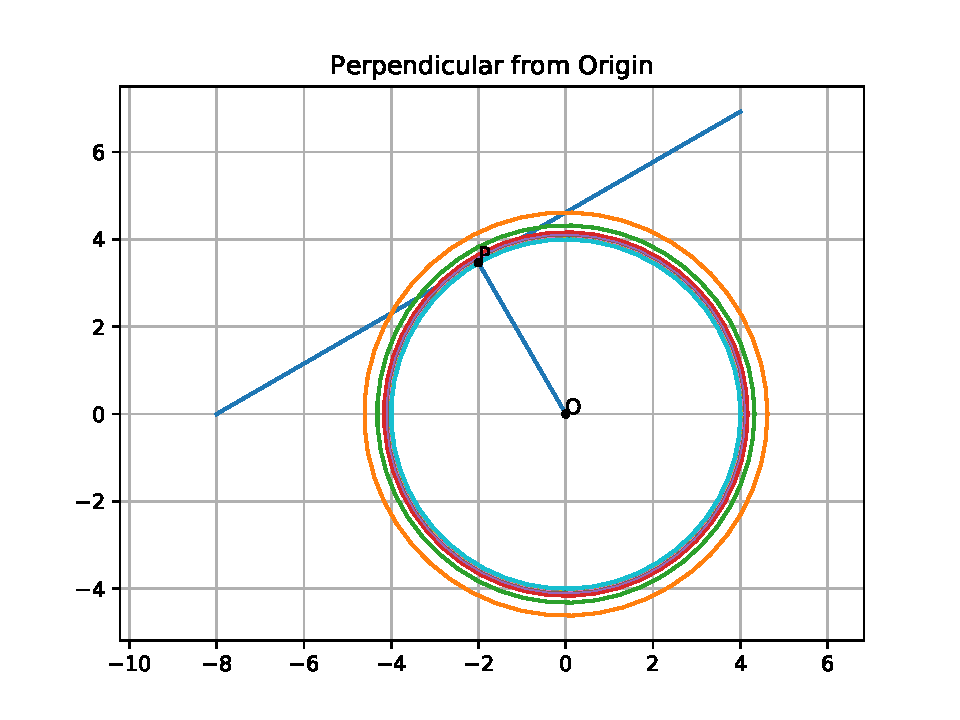
\includegraphics[width=\columnwidth]{11/10/3/3/1/lagmul/figs/problem3.1.pdf}
	\end{center}
\caption{}
\label{fig:11/10/3/3/1/lagmul/Fig1}
\end{figure}
